%-*-latex-*-
\sectionthree{Application: prefix tree}
\begin{python0}
from solutions import *; clear()
\end{python0}

A \defone{prefix tree} or a \defone{trie} is a tree for storing data with
lots of common prefixes.
What instance the word \texttt{cat} and \texttt{cab}
share a common prefix of \texttt{ca}.

As an example, say I want to store a list of words
in lowercase.
I use this
\begin{console}
class Node
{
public:
    char flag;
    Node * v[26];
};
\end{console}
Note that each node has 26 pointers, i.e., 26 edges going
to 26 children, each pointer corresponding to one fo the lower case letter.
Say I want to store the words \texttt{cab}, \texttt{cat}, \texttt{catch}.
Here's the picture:
\begin{center}
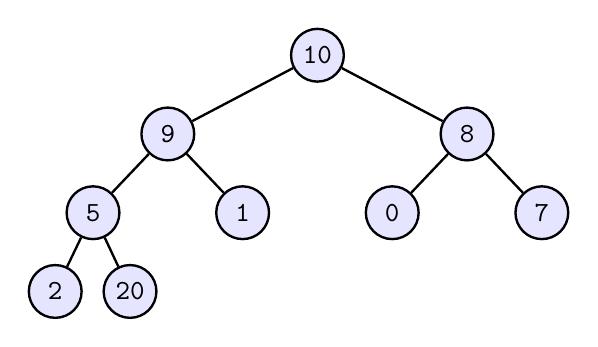
\begin{tikzpicture}

\fill[blue!10] (0.0, 0.0) circle (0.35);
\node [line width=0.03cm,black,minimum size=0.6699999999999999cm,draw,circle] at (0.0,0.0)(10){};\draw (0.0, 0.0) node[color=black] {\texttt{10}};
\fill[blue!10] (-1.9, -1.0) circle (0.35);
\node [line width=0.03cm,black,minimum size=0.6699999999999999cm,draw,circle] at (-1.9,-1.0)(9){};\draw (-1.9, -1.0) node[color=black] {\texttt{9}};
\fill[blue!10] (1.9, -1.0) circle (0.35);
\node [line width=0.03cm,black,minimum size=0.6699999999999999cm,draw,circle] at (1.9,-1.0)(8){};\draw (1.9, -1.0) node[color=black] {\texttt{8}};
\fill[blue!10] (-2.85, -2.0) circle (0.35);
\node [line width=0.03cm,black,minimum size=0.6699999999999999cm,draw,circle] at (-2.85,-2.0)(5){};\draw (-2.85, -2.0) node[color=black] {\texttt{5}};
\fill[blue!10] (-0.95, -2.0) circle (0.35);
\node [line width=0.03cm,black,minimum size=0.6699999999999999cm,draw,circle] at (-0.95,-2.0)(1){};\draw (-0.95, -2.0) node[color=black] {\texttt{1}};
\fill[blue!10] (0.95, -2.0) circle (0.35);
\node [line width=0.03cm,black,minimum size=0.6699999999999999cm,draw,circle] at (0.95,-2.0)(0){};\draw (0.95, -2.0) node[color=black] {\texttt{0}};
\fill[blue!10] (2.85, -2.0) circle (0.35);
\node [line width=0.03cm,black,minimum size=0.6699999999999999cm,draw,circle] at (2.85,-2.0)(7){};\draw (2.85, -2.0) node[color=black] {\texttt{7}};
\fill[blue!10] (-3.33, -3.0) circle (0.35);
\node [line width=0.03cm,black,minimum size=0.6699999999999999cm,draw,circle] at (-3.33,-3.0)(2){};\draw (-3.33, -3.0) node[color=black] {\texttt{2}};
\fill[blue!10] (-2.38, -3.0) circle (0.35);
\node [line width=0.03cm,black,minimum size=0.6699999999999999cm,draw,circle] at (-2.38,-3.0)(20){};\draw (-2.38, -3.0) node[color=black] {\texttt{20}};\draw[line width=0.03cm,black] (10) to  (9);
\draw[line width=0.03cm,black] (10) to  (8);
\draw[line width=0.03cm,black] (9) to  (5);
\draw[line width=0.03cm,black] (9) to  (1);
\draw[line width=0.03cm,black] (8) to  (0);
\draw[line width=0.03cm,black] (8) to  (7);
\draw[line width=0.03cm,black] (5) to  (2);
\draw[line width=0.03cm,black] (5) to  (20);
\end{tikzpicture}

\end{center}


What this means is that from the root node, say I call it
\verb!r!, there's an edge corresponding
to a pointer \verb!r.v[2]! (2 corresponding to \texttt{c})
that points to a node, say I call it \texttt{s}.
\texttt{s.v[0]} (0 corresponding to \texttt{a})
pointing to a node, say I call it \texttt{t}.
Etc.
If the node's flag is \texttt{*}, then it means that
I've reached a word when I start from the root.

When I draw this this edge between the lowest two nodes:

\begin{center}
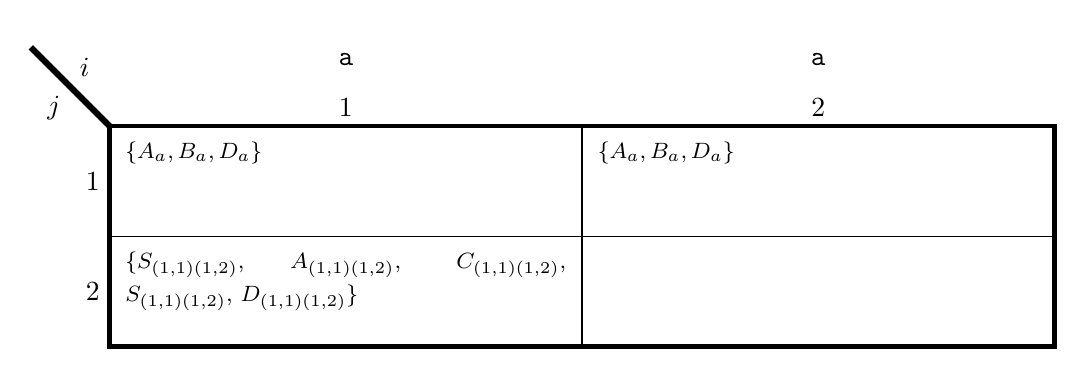
\begin{tikzpicture}

\draw (3.0, -0.7)
  node[draw, , , color=black,
       rounded corners=0cm, inner sep=0.2cm] {

\begin{minipage}[t][1.0cm]{5.6cm}
\mbox{}

\end{minipage}

};
\draw (3.0, -0.7) node[color=black,
 inner sep=0.2cm] {
 
\begin{minipage}[t][1.0cm]{5.6cm}
{\footnotesize $\{A_a,B_a,D_a\}$}
\end{minipage}

};
\draw (9.0, -0.7)
  node[draw, , , color=black,
       rounded corners=0cm, inner sep=0.2cm] {

\begin{minipage}[t][1.0cm]{5.6cm}
\mbox{}

\end{minipage}

};
\draw (9.0, -0.7) node[color=black,
 inner sep=0.2cm] {
 
\begin{minipage}[t][1.0cm]{5.6cm}
{\footnotesize $\{A_a,B_a,D_a\}$}
\end{minipage}

};
\draw (3.0, -2.0999999999999996)
  node[draw, , , color=black,
       rounded corners=0cm, inner sep=0.2cm] {

\begin{minipage}[t][1.0cm]{5.6cm}
\mbox{}

\end{minipage}

};
\draw (3.0, -2.0999999999999996) node[color=black,
 inner sep=0.2cm] {
 
\begin{minipage}[t][1.0cm]{5.6cm}
{\footnotesize $\{S_{(1,1)(1,2)},$ $A_{(1,1)(1,2)}$, $C_{(1,1)(1,2)}$, $S_{(1,1)(1,2)}$, $D_{(1,1)(1,2)} \}$}
\end{minipage}

};
\draw (9.0, -2.0999999999999996)
  node[draw, , , color=black,
       rounded corners=0cm, inner sep=0.2cm] {

\begin{minipage}[t][1.0cm]{5.6cm}
\mbox{}

\end{minipage}

};
\draw (9.0, -2.0999999999999996) node[color=black,
 inner sep=0.2cm] {
 
\begin{minipage}[t][1.0cm]{5.6cm}
{\footnotesize }
\end{minipage}

};\node[anchor=south] at (3.0,0.0) {1};\node[anchor=south] at (9.0,0.0) {2};\node[anchor=east] at (0,-0.7) {1};\node[anchor=east] at (0,-2.0999999999999996) {2};
\draw (6.0, -1.4)
  node[draw, line width=0.06cm, , color=black,
       rounded corners=0cm, inner sep=0cm] {

\begin{minipage}[t][2.8cm]{12.0cm}
\mbox{}

\end{minipage}

};\draw[line width=0.08cm,black] (0,0.0) to  (-1,1.0);
\node[anchor=north east] at (-0.5,0.5) {$j$};\node[anchor=south west] at (-0.5,0.5) {$i$};
\draw (3.0, 0.85)
  node[draw, line width=0.1cm, , color=white,
       rounded corners=0cm, inner sep=0cm] {

\begin{minipage}[t][0.7cm]{6.0cm}
\mbox{}

\end{minipage}

};\draw (3.0, 0.85) node[color=black] {{\texttt{a}}};
\draw (9.0, 0.85)
  node[draw, line width=0.1cm, , color=white,
       rounded corners=0cm, inner sep=0cm] {

\begin{minipage}[t][0.7cm]{6.0cm}
\mbox{}

\end{minipage}

};\draw (9.0, 0.85) node[color=black] {{\texttt{a}}};
\end{tikzpicture}

\end{center}


I mean this:

\begin{center}
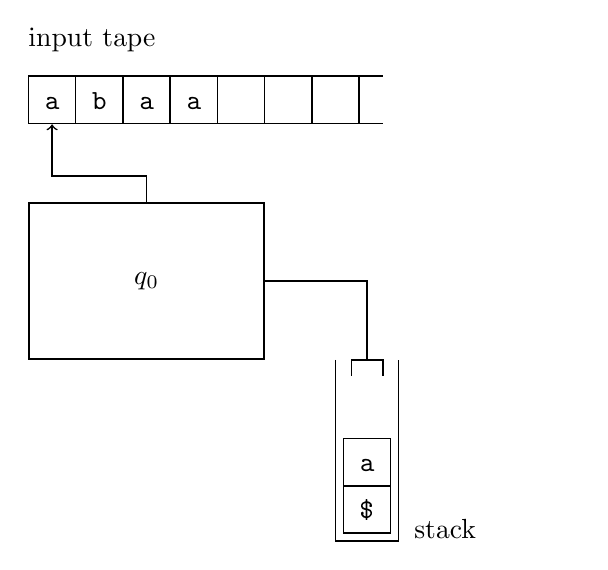
\begin{tikzpicture}

\draw (0.3, 0.3)
  node[draw, line width=0.02cm, , color=black,
       rounded corners=0cm, inner sep=0cm] {

\begin{minipage}[t][0.6cm]{0.6cm}
\mbox{}

\end{minipage}

};\draw (0.3, 0.3) node[color=black] {{\vphantom{a\$abaa\SPACE\SPACE\SPACE}\texttt{a}}};
\draw (0.8999999999999999, 0.3)
  node[draw, line width=0.02cm, , color=black,
       rounded corners=0cm, inner sep=0cm] {

\begin{minipage}[t][0.6cm]{0.6cm}
\mbox{}

\end{minipage}

};\draw (0.8999999999999999, 0.3) node[color=black] {{\vphantom{a\$abaa\SPACE\SPACE\SPACE}\texttt{b}}};
\draw (1.5, 0.3)
  node[draw, line width=0.02cm, , color=black,
       rounded corners=0cm, inner sep=0cm] {

\begin{minipage}[t][0.6cm]{0.6cm}
\mbox{}

\end{minipage}

};\draw (1.5, 0.3) node[color=black] {{\vphantom{a\$abaa\SPACE\SPACE\SPACE}\texttt{a}}};
\draw (2.0999999999999996, 0.3)
  node[draw, line width=0.02cm, , color=black,
       rounded corners=0cm, inner sep=0cm] {

\begin{minipage}[t][0.6cm]{0.6cm}
\mbox{}

\end{minipage}

};\draw (2.0999999999999996, 0.3) node[color=black] {{\vphantom{a\$abaa\SPACE\SPACE\SPACE}\texttt{a}}};
\draw (2.7, 0.3)
  node[draw, line width=0.02cm, , color=black,
       rounded corners=0cm, inner sep=0cm] {

\begin{minipage}[t][0.6cm]{0.6cm}
\mbox{}

\end{minipage}

};\draw (2.7, 0.3) node[color=black] {{\vphantom{a\$abaa\SPACE\SPACE\SPACE}\texttt{\SPACE}}};
\draw (3.3, 0.3)
  node[draw, line width=0.02cm, , color=black,
       rounded corners=0cm, inner sep=0cm] {

\begin{minipage}[t][0.6cm]{0.6cm}
\mbox{}

\end{minipage}

};\draw (3.3, 0.3) node[color=black] {{\vphantom{a\$abaa\SPACE\SPACE\SPACE}\texttt{\SPACE}}};
\draw (3.9000000000000004, 0.3)
  node[draw, line width=0.02cm, , color=black,
       rounded corners=0cm, inner sep=0cm] {

\begin{minipage}[t][0.6cm]{0.6cm}
\mbox{}

\end{minipage}

};\draw (3.9000000000000004, 0.3) node[color=black] {{\vphantom{a\$abaa\SPACE\SPACE\SPACE}\texttt{\SPACE}}};\draw[line width=0.02cm,black] (4.199999999999999,0.6) to  (4.5,0.6);
\draw[line width=0.02cm,black] (4.199999999999999,0.0) to  (4.5,0.0);

\draw (3.0, 1.1)
  node[draw=none, line width=0cm, , color=black,
       rounded corners=0cm, inner sep=0cm] {

\begin{minipage}[t][0.1cm]{6cm}
\mbox{}

\end{minipage}

};
\draw (3.0, 1.1) node[color=black,
 inner sep=0cm] {
 
\begin{minipage}[t][0.1cm]{6cm}
input tape
\end{minipage}

};
\draw (1.5, -2.0)
  node[draw, line width=0.02cm, , color=black,
       rounded corners=0cm, inner sep=0cm] {

\begin{minipage}[t][1.98cm]{2.98cm}
\mbox{}

\end{minipage}

};\draw (1.5, -2.0) node[color=black] {$q_0$};\draw[line width=0.02cm,black,->] (1.5,-1) to  (1.5,-0.67) to  (0.3,-0.67) to  (0.3,-0.01);

\draw (4.3, -4.3)
  node[draw, line width=0.02cm, , color=black,
       rounded corners=0cm, inner sep=0cm] {

\begin{minipage}[t][0.6cm]{0.6cm}
\mbox{}

\end{minipage}

};\draw (4.3, -4.3) node[color=black] {{\vphantom{a\$abaa\SPACE\SPACE\SPACE}\texttt{a}}};
\draw (4.3, -4.8999999999999995)
  node[draw, line width=0.02cm, , color=black,
       rounded corners=0cm, inner sep=0cm] {

\begin{minipage}[t][0.6cm]{0.6cm}
\mbox{}

\end{minipage}

};\draw (4.3, -4.8999999999999995) node[color=black] {{\vphantom{a\$abaa\SPACE\SPACE\SPACE}\texttt{\$}}};\draw[line width=0.02cm,black] (3.9,-3.0) to  (3.9,-5.3) to  (4.7,-5.3) to  (4.7,-3.0);

\draw (5.949999999999999, -5.1499999999999995)
  node[draw=none, line width=0cm, , color=black,
       rounded corners=0cm, inner sep=0cm] {

\begin{minipage}[t][0.1cm]{2.1cm}
\mbox{}

\end{minipage}

};
\draw (5.949999999999999, -5.1499999999999995) node[color=black,
 inner sep=0cm] {
 
\begin{minipage}[t][0.1cm]{2.1cm}
stack
\end{minipage}

};\draw[line width=0.02cm,black] (3,-2.0) to  (4.3,-2.0) to  (4.3,-3.0);
\draw[line width=0.02cm,black] (4.1,-3.2) to  (4.1,-3.0) to  (4.5,-3.0) to  (4.5,-3.2);
\end{tikzpicture}

\end{center}



i.e., each node has a character and a vector of 26 pointers.
The node at the top has a character value of \verb!' '! and for the vector
of pointers, 25 of them at \texttt{NULL} while the
pointer at index 7 (which corresponds to character \texttt{h})
points to the next node which contains a character value of \texttt{*}
a vector of 26 pointers, all of which are \texttt{NULL}.

Get it? Neat right?

Note that the prefix above is a 26-ary tree since
each edge corresponds to one of the lowecase letter.
(If you want lower and upper case, then it's a 52-ary tree.)

\begin{ex}
Build a prefix tree for \texttt{cab}, \texttt{cat} and
\texttt{catch} using the class above.
Do it with this function:
\begin{Verbatim}[frame=single]
void insert(Node ** p, const std::string & word);
\end{Verbatim}
Write a function that accepts a string (use
\texttt{std::string}) and checks if the word
is stored in the prefix tree.
In other words when you call the function with \texttt{cat}
it returns \texttt{true};
if you call the function with \texttt{cas} is returns \texttt{false}.
Here's an appropriate prototype:
\begin{Verbatim}[frame=single]
bool is_found(const Node * const, const std::string &);
\end{Verbatim}
\qed
\end{ex}

\begin{ex}
In case you added a wrong word, you want to be able to remove a
\lq\lq word''. So do this:
\begin{Verbatim}[frame=single]
void delete(Node ** p; const std::string & word);
\end{Verbatim}
Fail silently, i.e., if you attempt to delete a word not in the
prefix tree, don't throw an exception.
Also, reclaim memory as much as you can. For instance in the above
prefix tree:
\begin{center}
\begin{tikzpicture}

\fill[white] (0.0, 0.0) circle (0.4);
\node [line width=0.03cm,black,minimum size=0.77cm,draw,circle] at (0.0,0.0)(1){};\draw (0.0, 0.0) node[color=black] {$p$};
\fill[white] (5.0, 0.0) circle (0.4);
\node [line width=0.03cm,black,minimum size=0.77cm,draw,circle] at (5.0,0.0)(2){};\draw (5.0, 0.0) node[color=black] {$q$};\draw[line width=0.03cm,black,->,>=triangle 60] (1) to node [above] {$\texttt{a}, \texttt{b} \rightarrow \texttt{c} $} (2);
\end{tikzpicture}

\end{center}


if you delete the word \texttt{catch}, the
memory model of the prefix tree should be

\begin{center}

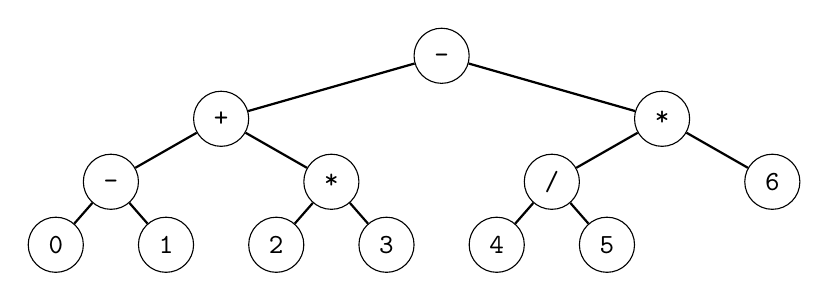
\begin{tikzpicture}
\node at (4.8999999999999995,-0.8) [circle,draw,minimum size=7mm] (A) {\texttt{-}};
\node at (2.0999999999999996,-1.6) [circle,draw,minimum size=7mm] (B) {\texttt{+}};
\node at (7.699999999999999,-1.6) [circle,draw,minimum size=7mm] (C) {\texttt{*}};
\node at (0.7,-2.4000000000000004) [circle,draw,minimum size=7mm] (D) {\texttt{-}};
\node at (3.5,-2.4000000000000004) [circle,draw,minimum size=7mm] (E) {\texttt{*}};
\node at (6.3,-2.4000000000000004) [circle,draw,minimum size=7mm] (F) {\texttt{/}};
\node at (9.1,-2.4000000000000004) [circle,draw,minimum size=7mm] (G) {\texttt{6}};
\node at (0.0,-3.2) [circle,draw,minimum size=7mm] (H) {\texttt{0}};
\node at (1.4,-3.2) [circle,draw,minimum size=7mm] (I) {\texttt{1}};
\node at (2.8,-3.2) [circle,draw,minimum size=7mm] (J) {\texttt{2}};
\node at (4.199999999999999,-3.2) [circle,draw,minimum size=7mm] (K) {\texttt{3}};
\node at (5.6,-3.2) [circle,draw,minimum size=7mm] (L) {\texttt{4}};
\node at (7.0,-3.2) [circle,draw,minimum size=7mm] (M) {\texttt{5}};
\draw [-,thick] (A) -- (B);
\draw [-,thick] (A) -- (C);
\draw [-,thick] (B) -- (D);
\draw [-,thick] (B) -- (E);
\draw [-,thick] (C) -- (F);
\draw [-,thick] (C) -- (G);
\draw [-,thick] (D) -- (H);
\draw [-,thick] (D) -- (I);
\draw [-,thick] (E) -- (J);
\draw [-,thick] (E) -- (K);
\draw [-,thick] (F) -- (L);
\draw [-,thick] (F) -- (M);

;
\end{tikzpicture}
    
\end{center}


In particular, the node that the edge labeled \texttt{t} reaches
has a vector of 26 \verb!NULL! pointers.
It's not enough just to make the character in the node that the
ledge labeled \texttt{h} leads to with a space.
\qed
\end{ex}

Because words in English (and many other languages too)
contains lots of common prefixes,
this is a very efficient way of storing words
and therefore can be used to create dictionaries.

Not only that, this is also how
word autocompletion works inside programs.
If you type part of a word into a software, the program
can sometimes give you a list of options to complete the word
once the number of options is small enough.
How does it know?
Well, as you type, the program walks down the above
tree.
From where you stop typing,
it can perform a traversal of the subtree where
the root corresponds to where you stopped.
In the traversal, when it sees a \texttt{*}
it knows that it's a word (from the root of the subtree to that node). 
Therefore the program can collect a list of
words with the same prefix as what you have typed.
The program then shows you the options.
Neat right?

\begin{ex}
Continuing the above
exercise,
write a function that
gives you a list of word completion.
if you call the function with \texttt{ca}
it returns an array (use \texttt{std::vector})
containing \texttt{cat} and \texttt{catch}.
\qed
\end{ex}

\begin{ex}
Download a dictionary file from the web.
Convert all uppercase to lowercase.
How many bytes are there in the file.
Next, build a prefix tree and then compute the
amount of memory used.
How much memory do you save?
\qed
\end{ex}

Instead of having a vector for pointers where there's one pointer
\textit{every} character \texttt{a..z},
you can have a vector of (character, pointer)  only for characters that
are actually used.
In that case the root node in the above prefix tree has only
one pointer and not 26.
However this will slow you down when you look for the word.
You can use a sorted \texttt{std::vector} to speed up the search.
This will of course save you on memory.
This is again the story of the life of algorithms:
it's always about the balance between speed and memory.
